%%
%% This is file `mcmthesis-demo.tex',
%% generated with the docstrip utility.
%%
%% The original source files were:
%%
%% mcmthesis.dtx  (with options: `demo')
%% !Mode:: "TeX:UTF-8"
%% -----------------------------------
%%
%% This is a generated file.

%%
%% This work may be distributed and/or modified under the
%% conditions of the LaTeX Project Public License, either version 1.3
%% of this license or (at your option) any later version.
%% The latest version of this license is in
%%   http://www.latex-project.org/lppl.txt
%% and version 1.3 or later is part of all distributions of LaTeX
%% version 2005/12/01 or later.
%%
%% This work has the LPPL maintenance status `maintained'.
%%
%% The Current Maintainer of this work is Liam Huang.
%%
\documentclass[12pt]{mcmthesis}
\mcmsetup{CTeX = true,   % 使用 CTeX 套装时,设置为 true
        tcn = \textcolor[rgb]{0,0.00,0.00}{1924935}, problem = \textcolor[rgb]{0,0.00,0.00}{C},
        sheet = true, titleinsheet = true, keywordsinsheet = true,
        titlepage = false, abstract = true}
\usepackage{palatino}
\usepackage{lipsum}
\usepackage{longtable}
\usepackage{graphicx, subfig}
\title{Multi-algorithm Combined Model for Dealing with Abuse of Opioids}
\author{}
\date{}

\makeatletter
\renewcommand*\l@section{\@dottedtocline{1}{12pt}{12pt}}
%\makeatother
\begin{document}
\begin{abstract}
The abuse of addictive opioids has brought unprecedented challenges. We conducted an analysis to  solve this problem better.\par
For part 1, we first refer to \textbf{the SIR model} and propose a propagation characteristic analysis model. \textbf{The result is that } synthetic opioids and heroin both tend to grow in high-volume areas and spread to low-volume areas. Then, we combined \textbf{the entropy method} and \textbf{the ARIMA model} to propose a predictive model for drug abuse in the state. To analyze the county more easily, we use \textbf{principal component analysis} to analyze it.\textbf{ The result is:} in 2018,HAMILTON(39061) is the most prone to abuse of synthetic opioids, CUYAHOGA(39035) is second, MONTGOMERY(39113) is third; MONTGOMERY(39113) is the most prone to heroin abuse, followed by LAKE(39085), and the third is LUCAS(39095).When this situation continues, after 2022, when the total number of drug abuses in Ohio (39) reached \textbf{the threshold} of 275,040, both synthetic opioids and heroin suddenly exploded.\par
For part 2,through \textbf{the BP neural algorithm},we find several items with larger weights in each indicator. \textbf{The result is:}divorced men, low-educated people, and separated men  likely that they are likely to abuse opioids.\par
For Part 3,we have proposed some solutions to the opioids crisis and verified the feasibility of these solutions through the model.\par
In addition, we also verified the model. When using 2017-2016 data to predict 2017, \textbf{the average relative error is 7.757\%}, and the accuracy of the model is high.\par
We also analyzed the advantages and disadvantages of the model and gave the improvement aspects.
\setlength{\parindent}{0pt}
\begin{keywords}
Synthetic Opioids and Herion;ARIMA;BP neural algorithm;Opioids Crisis
\end{keywords}
\end{abstract}
\maketitle

\tableofcontents
\newpage

\section{Introduction}
\subsection{Background}
The abuse of opioids is increasingly becoming a cause of hindering the health of the American people.Even economically, opioid may become a lack of talent in certain important neighborhoods of the United States by making people with high academic qualifications addicted, thereby affecting the economy.At the same time, a large number of opioid addicts will also put a heavy pressure on the medical system.\par Therefore, it is necessary to find out the causes and objects of abuse of opioids and stop such abuse in time.
\subsection{Restatement of the Problem}
In the face of the increasingly serious opioids abuse situation, combined with the existing information, considering the five states of Ohio, Kentucky, West Virginia, Virginia, and Pennsylvania,we need to complete the following:
\begin{enumerate}
\item Use the data provided by the NFLIS to create a mathematical model that describes the propagation characteristics of synthetic opioids and heroin over time between the five states and their counties.At the same time, identify the locations in the five states that may have begun to use specific opioids.\\After that,given a threshold, elaborate what will happen when this threshold is reached ,which the US government should be concerned , and use the model to predict when and where the threshold will be reached.
\item Use the data provided by the U.S. Census socio-economic to improve the previous model and use reasonable assumptions to explain which factors are related to the abuse of opioids.
\item Combine the results of previous models to determine a viable solution to the opioid crisis. Also check the feasibility of the program and identify factors that may lead to success or failure.
\end{enumerate}
\section{Assumptions and Justifications}
We make the following assumptions to approximate and simplify the problem.
\begin{enumerate}
  \item \textbf{The change of data with time is regular, and this law does not change in a short time. }This is the most fundamental condition for making predictions.
  \item \textbf{The reported data is the total occurrence value, that is to say, there is no case that drug abuse has occurred and is not reported.}Because the reported drug abuse should be positively related to what actually happened, so to some extent, the reported drug abuse can be used instead of the actual value.
  \item \textbf{Ignore the differences in the spread of different drugs between different regions.}This condition will make the calculation of the model simpler and easier to understand.
\item \textbf{Drugs produced in the region are allocated to local and other regions according to a fixed ratio.}This condition simplifies the calculation of the model.
\item \textbf{If the United States makes adjustments, it will only affect the production of drugs.}This condition makes the model more reasonable, because it is also the main regulation of the state in the actual operation process.
\end{enumerate}

Besides these general assumptions, there are also hypotheses we make for the specific models.We will present and discuss them inspecific model.

\section{Symbol Description}
\begin{table}[htbp]
 \centering
    \caption{Notations}\label{Notations}
  \begin{tabular}{c|c}
     \hline
     Symbol & Meaning \\\hline
     $S(t)$ & the Amount of drug \\
     $P(t)$ &the Amount of
drug Produced\\
$I(t)$& the Number of drugs Shipped from other Regions\\
$\varepsilon$&the Adjustment Factor \\
$\theta$&the
Acceptance Rate of drugs\\
$\eta$&The Rate of Adjustment\\
$C$&Contribution Rate\\
     $W$ & Weight or Weight Matrix \\
     \hline
   \end{tabular}
\end{table}


\section{Model 1:Propagation Analysis and Prediction Model}

\subsection{Propagation Analysis Model based on SIR model}
In this model, we add a new hypothesis:\textbf{This year's local production value is only adjusted by the local occurrence value of the previous year, ignoring the influence of other years and other regions.}This condition makes us not have to consider the complicated calculations brought by multi-regional effects.
\subsubsection{Preparation of Analysis Model}
According to the Wikipedia\cite{wiki}, we classify opioids, the results are shown in Table \ref{table:opioid} (in the appendix).\par
According to the classification method of Table 1, the number of synthetic opioids and heroin in each state and county  can be obtained separately. Here, we present the synthetic opioids in Ohio (Table \ref{39state}) and the heroin situation in Kentucky (Table \ref{21state}).
\begin{table}[htb]
\centering
\caption{The situation of Synthetic Opioids in 39(Ohio)}\label{39state}
\begin{tabular}{|c|c|c|c|}
\hline
Year & Synthetic Opioids& Total&Proportion \\\hline
2010 & 757   & 70999  & 0.01 \\
2011 & 636   & 71282  & 0.01 \\
2012 & 525   & 85415  & 0.01 \\
2013 & 587   & 93747  & 0.01 \\
2014 & 1942  & 101423 & 0.02 \\
2015 & 5250  & 109150 & 0.05 \\
2016 & 12867 & 115276 & 0.11 \\
2017 & 23437 & 119349 & 0.20 \\\hline
\end{tabular}
\end{table}
\begin{table}[htb]
\centering
\caption{The situation of heroin in 21(Kentucky)}\label{21state}
\begin{tabular}{|c|c|c|c|}
\hline
Year & Herion& Total&Proportion \\\hline
2010 & 629  & 29588 & 0.02 \\
2011 & 899  & 28285 & 0.03 \\
2012 & 2320 & 27502 & 0.08 \\
2013 & 4175 & 26820 & 0.16 \\
2014 & 4362 & 27077 & 0.16 \\
2015 & 4045 & 25811 & 0.16 \\
2016 & 3716 & 26530 & 0.14 \\
2017 & 3231 & 28870 & 0.11 \\\hline
\end{tabular}
\end{table}
In each table, we consider the number of abused opioids (synthetic synthetic opioids or heroin), the total amount of drug use in the year, and the proportion between the two as a function of time.
\par Next, we discuss the propagation characteristics of synthetic opioids and heroin.
\subsubsection{Establishment of Analysis Model}
 Suppose S(t) is the amount of drug in a particular region, P(t) is the amount of drug produced in the region, and the ratio of local to other regions is assumed to be m: (1-m).\par I(t) is the number of drugs shipped from other regions.\par $\varepsilon$ is the adjustment factor of national macro policy to production.
$\theta$ is the acceptance rate of drugs produced in other regions.
The rate of adjustment of the number of local drugs in the previous year to this year's production is $\eta$.\par
Through the principle of the SIR model\cite{computer virus}, the relationship between the production amount P and the local drug amount S is obtained as Equation (\ref{produce1})
\begin{equation}\label{produce1}
\left\{
\begin{array}{c}
  P(t)=S(t-1)\cdot\frac{1+\eta}{1+\varepsilon}\\
  S(t)=mP(t)+\theta I(t)\\
  \end{array}
  \right.
\end{equation}
By Equation (\ref{produce1}) , there is:
\begin{equation}\label{all1}
  S(t)=S(t-1)\cdot m \frac{1+\eta}{1+\varepsilon}+\theta I(t)
\end{equation}
Differential for Equation (\ref{all1}), there is:
\begin{equation}\label{all2}
\frac{dS(t)}{dt}=m\frac{1+\eta}{1+\varepsilon} dS(t-1)+\theta\cdot \frac{dI(t)}{dt}
\end{equation}
\subsubsection{Results of Analysis Model}
With Equation (\ref{all2}), the data is brought into MATLAB to draw a 3D surface map. Among them, the propagation of synthetic opioids and heroin between states is shown in Figure \ref{opioids}.In the figure, 1-5 represents the corresponding State (21, 39, 42, 51, 54).
\begin{figure}[htbp]
\centering
\begin{tabular}{cc}
 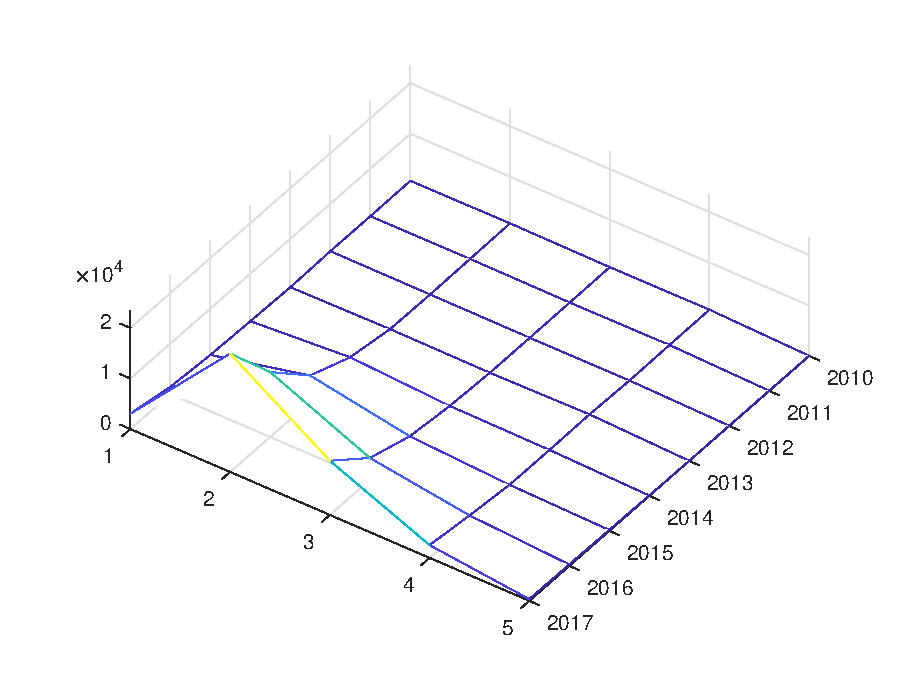
\includegraphics[width=0.5\textwidth]{figures/synthetic.eps} &   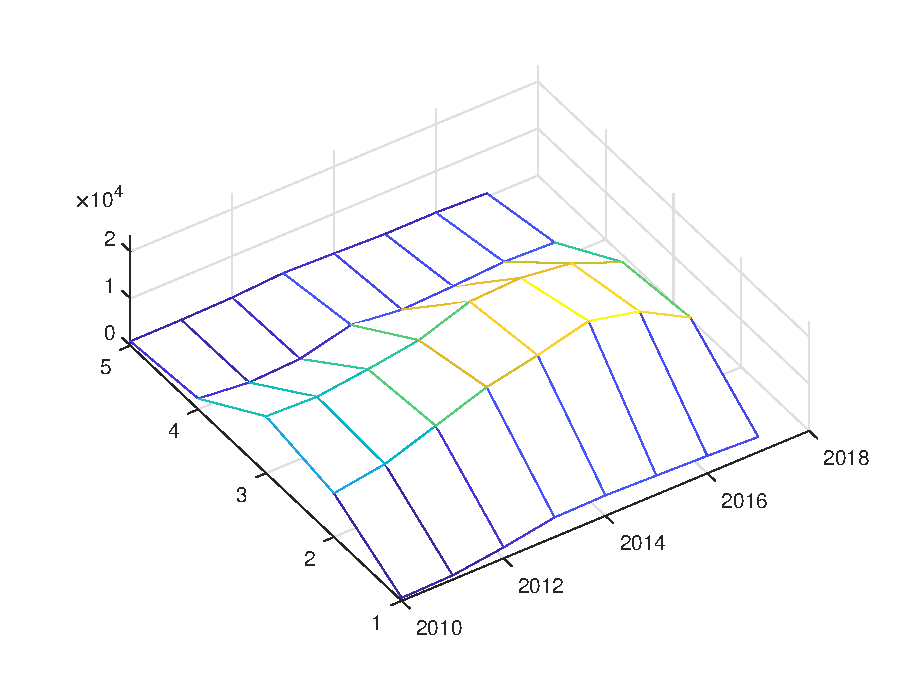
\includegraphics[width=0.5\textwidth]{figures/herion.eps}\\
 Synthetic Opioids&Heroin\\
\end{tabular}
  \caption{Propagation Characteristics of Opioids}\label{opioids}
\end{figure}\par
It can be seen from the figure that the synthetic opioid and heroin have similar propagation characteristics, which are transmitted from a high concentration area to a low concentration area, while the concentration of high concentration area tends to be higher.
\subsection{Prediction Model Combined with Entropy Method and ARIMA }
With the propagation model, we get the propagation properties of opioids. From this, we can predict where the abuse of opioids is most likely to occur and calculate the threshold.
\subsubsection{Establishment of Prediction Model}
\paragraph{Entropy Method}
In information theory, entropy is a measure of uncertainty\cite{weight}. The larger the amount of information, the smaller the uncertainty and the smaller the entropy. According to the characteristics of entropy, we can calculate the degree of dispersion of a project by calculating the entropy value. The greater the degree of dispersion of the project, the greater the impact on the comprehensive evaluation.\par
Select $n$ states, $m$ years, then $x_{ij}$ is the value of the $i$-th state of the $j$-th year.\par
Standardize each year:
\begin{equation}
 x'_{ij}=\left[\frac{\left|x_{ij}\right|-\min\left(\left|x_{1j}\right|,\left|x_{2j}\right|,\dotsm,\left|x_{nj}\right|\right)}{\max\left(\left|x_{1j}\right|,\left|x_{2j}\right|,\dotsm,\left|x_{nj}\right|\right)-\min\left(\left|x_{1j}\right|,\left|x_{2j}\right|,\dotsm,\left|x_{nj}\right|\right)}\right]\times 100
\end{equation}\label{shangzhi}
Calculate the proportion of the $i$-th state in the year $j$:
\begin{equation}
p_{ij}=\frac{x'_{ij}}{\sum_{i=1}^n x'_{ij}}
\end{equation}
Calculate the entropy of the $j$-th year:
\begin{equation}
e_j=-k\sum_{i=1}^{n}p_{ij}\ln\left(p_{ij}\right)
\end{equation}
where
$k=\frac{1}{\ln\left(n\right)}$.\\
Calculate the coefficient of variation for the $j$-th year. For the $j$-th year, the larger the variation, the smaller the entropy value. Define the coefficient of variation:
\begin{equation}
g_j=\frac{1-e_j}{m-E_e}
\end{equation}
where
$E_e=\sum_{j=1}^{m}e_j$.\\
Calculate the weight:
\begin{equation}
w_j=\frac{g_j}{\sum_{j=1}^{m}g_j}
\end{equation}
Calculate the score for each state:
\begin{equation}
s_i=\sum_{j=1}^{m}w_j\cdot  p_{ij}
\end{equation}
\paragraph{ARIMA}
ARIMA is a common prediction method for analyzing time sequence\cite{ARIMA}. The model structure of ARIMA(p,d,q) is:
\begin{equation}
\left\{
\begin{array}{cc}
\Phi(B)\nabla^dy_t=\Theta(B)\varepsilon_t\\
E(\varepsilon_t)=0,Var(\varepsilon_t)=\sigma_{\varepsilon}^2,E(\varepsilon_t\varepsilon_s),&s\neq t\\
E(y_t\varepsilon_t)=0,&\forall s<t
\end{array}
\right.
\end{equation}
where
$\nabla^d=(1-B)^d$.\\
$\Phi(B)=1-\theta_1B-\dotsc-\theta_qB_q$ is the autoregressive coefficient polynomial in a stationary reversible ARMA(p,q) model;\\
$\Theta(B)=1-\theta_1B-\dotsc-\theta_qB_q$ is the moving smoothing coefficient polynomial in the stationary reversible ARMA(p,q) model.\\
And $\{\varepsilon_t\}$ is a zero mean white noise sequence.
\paragraph{Prediction Model}
In order to reduce the error, we use the entropy method to predict the weight of each state (county) and use ARIMA to predict the weight. Finally, a comprehensive analysis identifies the areas with the highest probability.\par
In the analysis of the proportion of the county, since there are many counties in each state, we use principal component analysis to analyze\cite{zhuchengfen}:\par If the sample data X is an n$\times$p matrix:
$$X=\left[
      \begin{array}{cccc}
        x_{11} & x_{12} & \cdots&x_{1p} \\
        x_{21} & x_{22} & \cdots& x_{2p}\\
        \vdots&\vdots& &\vdots\\
        x_{n1} & x_{n2} & \cdots&x_{np} \\
      \end{array}
    \right]
$$
Standardize the raw data:
\begin{equation}
\begin{array}{ccc}
  x_{ij}^*=\frac{x_{ij}-\bar{x}_j}{\sqrt{Var(x_j)}}&(i=1,2,\dotsc,n;j=1,2,\dotsc,p)
  \end{array}
\end{equation}
where
$ \bar{x_j}=\frac{1}{n}\sum_{i=1}^{n}x_{ij};Var(x_j)=\frac{1}{n-1}\sum_{i=1}^{n}(x_{ij}-\bar{x})^2(j=1,2,\dotsc,p)$\\
Calculating the sample correlation coefficient matrix:
$R=\left[
      \begin{array}{cccc}
        r_{11} & r_{12} & \cdots&r_{1p} \\
        r_{21} & r_{22} & \cdots& r_{2p}\\
        \vdots&\vdots& &\vdots\\
        r_{p1} & r_{p2} & \cdots&r_{pp} \\
      \end{array}
    \right]
$
\begin{equation}
r_{ij}=Cov(x_i^*,x_j^*)=\frac{\sum_{k=1}^{n}(x_i^*-\bar{x}_i)(x_j^*-\bar{x}_j)}{n-1},n>1
\end{equation}
Calculating the eigenvalue $\lambda_1,\lambda_2,\dotsc,\lambda_p$ of the correlation coefficient matrix R and the corresponding eigenvector
$a_i=(a_{i1},a_{i2},\dotsc,a_{ip}),i=1,2,\dotsc,p)$
Calculate the contribution rate of each principal component
\begin{equation}
C_i=\frac{\lambda_i}{\sum_{i=1}^{p}\lambda_i}
\end{equation}
Calculate the principal component score in the following form
$$F=\left[
      \begin{array}{cccc}
        f_{11} & f_{12} & \cdots&f_{1k} \\
        f_{21} & f_{22} & \cdots& f_{2k}\\
        \vdots&\vdots& &\vdots\\
        f_{n1} & f_{n2} & \cdots&f_{nk} \\
      \end{array}
    \right]
$$
\begin{equation}
f_{ij}=a_{j1}x_{i1}^*+a_{j2}x_{i2}^*+\dotsb+a_{jp}x_{ip}^*,i=1,2,\dotsc,n;j=1,2,\dotsc,k
\end{equation}
\subsubsection{Results of Prediction Model}
The entropy is calculated by EXCEL, and the Proportion is predicted by SPSS. The results of States are shown in Figure \ref{arimas} and Table \ref{results1},\ref{results12}, respectively. Where $W=Proportion\times Entropy $.(When predicting the proportion of synthetic opioids, we predict the number of each states and total number at the same time, and finally obtain the ratio. When predicting the proportion of heroin, it is directly predicted. These two methods are essentially identical.)\par
\begin{figure}
  \centering
  \begin{tabular}{cc}
    % after \\: \hline or \cline{col1-col2} \cline{col3-col4} ...
    \includegraphics[width=0.5\textwidth]{figures/synthetic_(1).eps}& 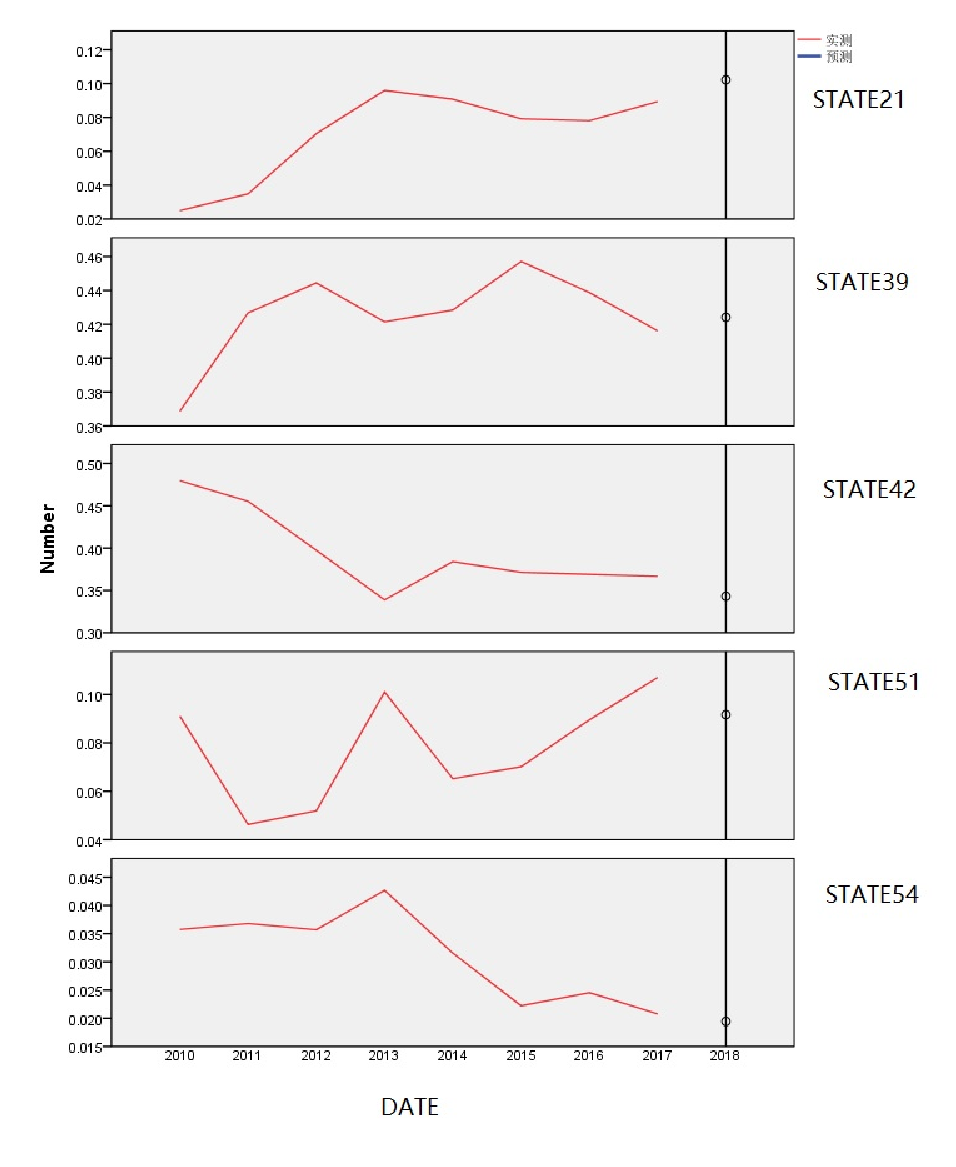
\includegraphics[width=0.5\textwidth]{figures/herion_(1).eps} \\
    Synthetic Opioids & Herion \\
  \end{tabular}
  \caption{Prediction Results of ARIMA Model }\label{arimas}
\end{figure}
%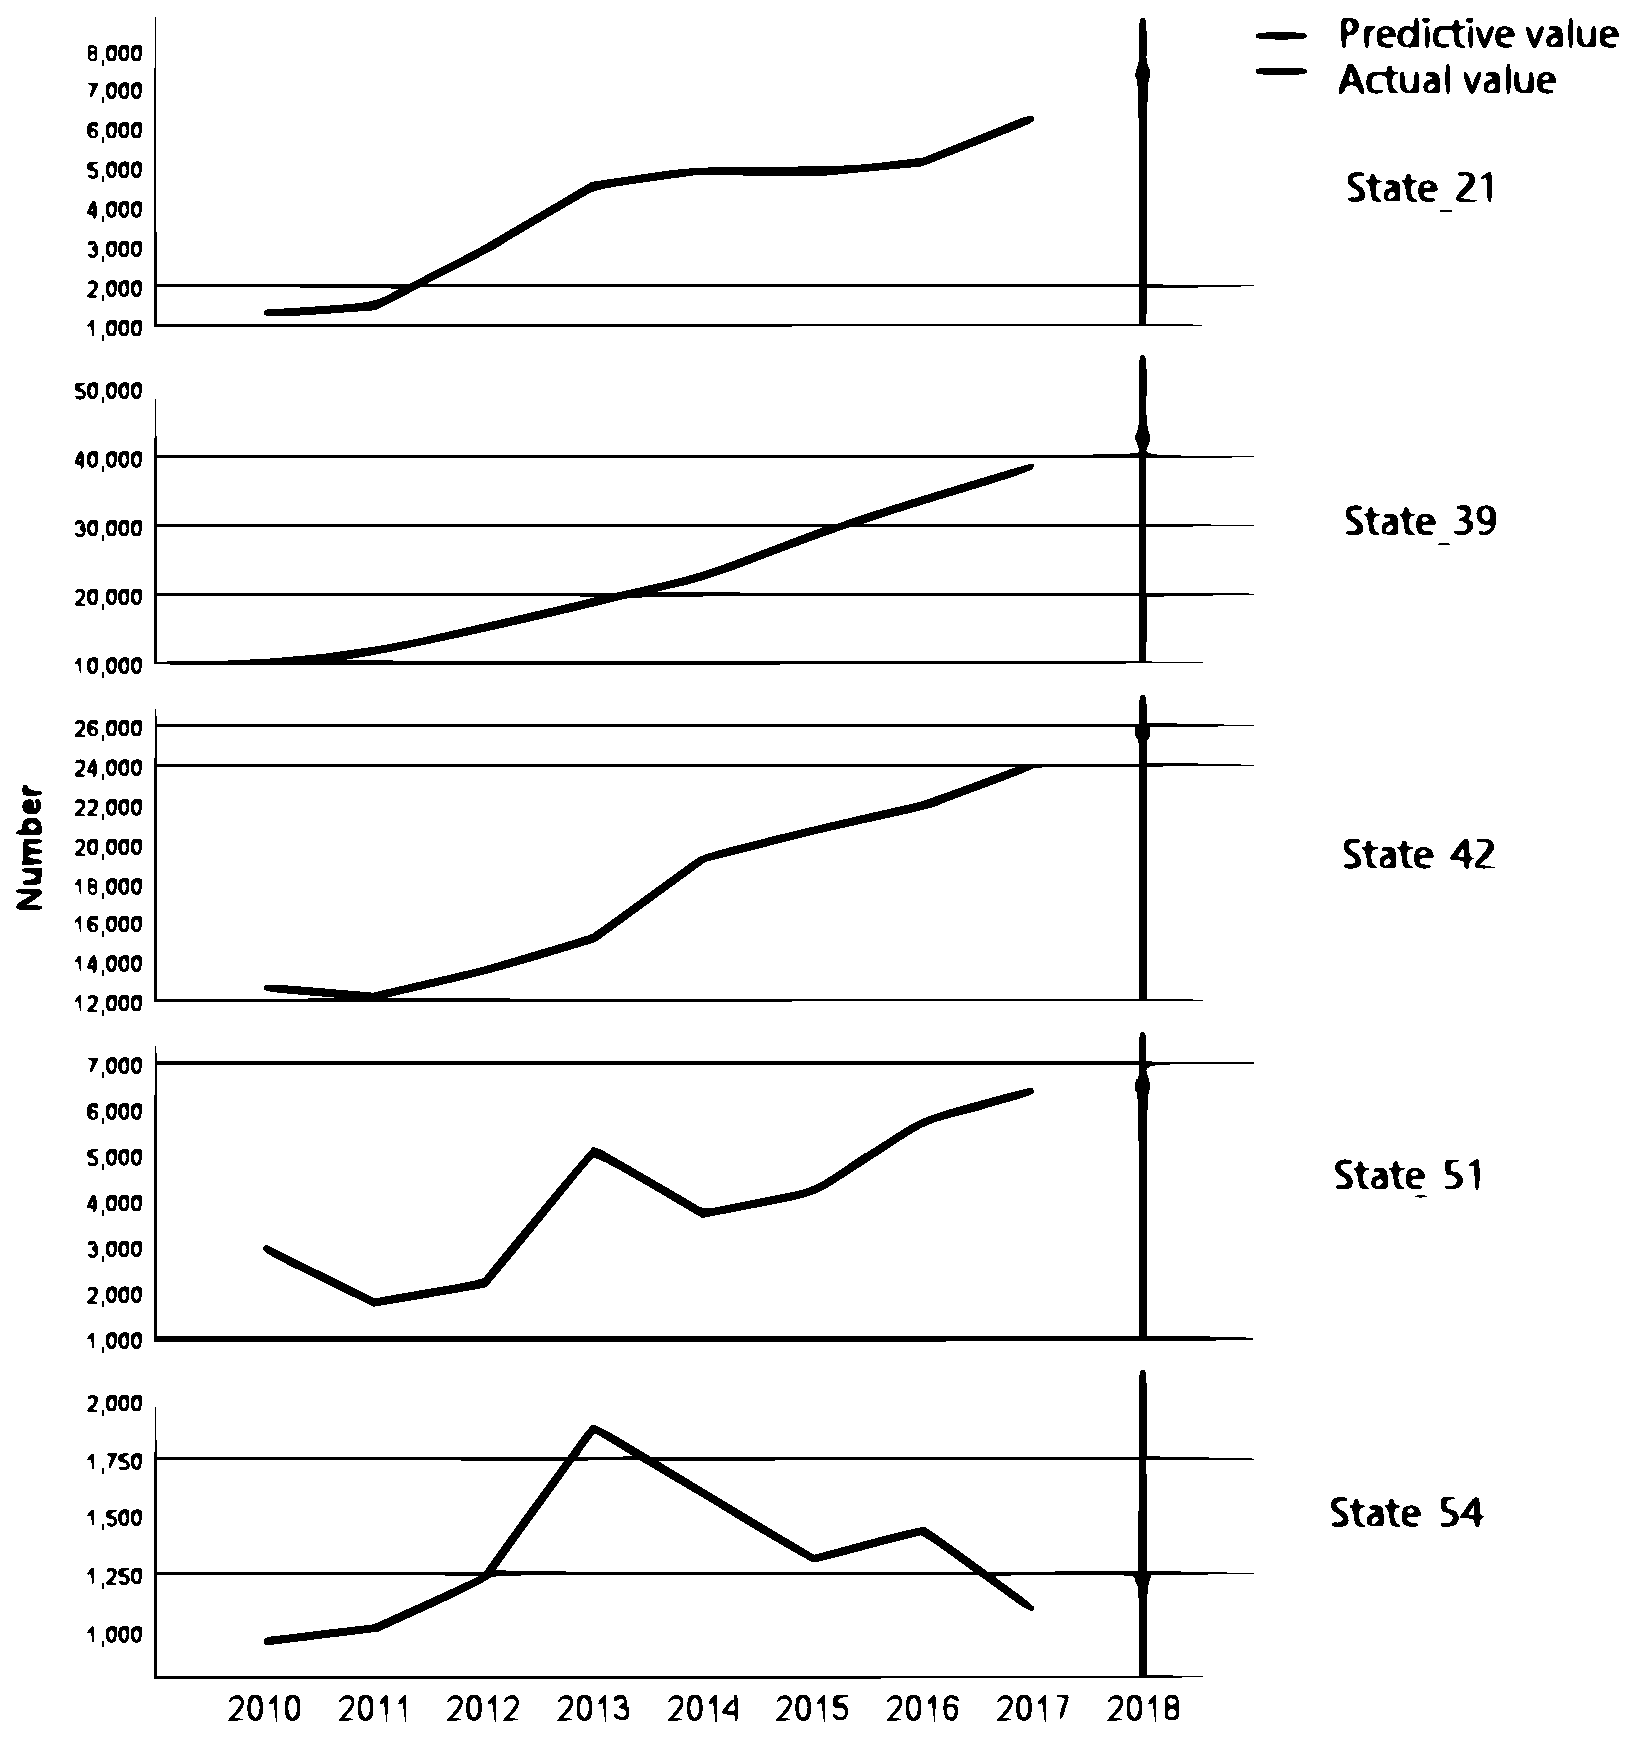
\includegraphics[width=0.5\textwidth]{figures/ARIMA.eps}
\begin{table}[htb]
\centering
\caption{Prediction Model Results for each State,Synthetic Opioids}\label{results1}
\begin{tabular}{|c|c|c|c|c|c|}
\hline
State      & 21        & 39         & 42        & 51        & 54       \\\hline
Proportion & 0.0733    & 0.5478     & 0.3039    & 0.0525    & 0.0064   \\\hline
Entropy    & 2158.0111 & 16629.7353 & 7160.8756 & 1876.2172 & 278.5188 \\\hline
W          & 158.1863  & 9110.2279  & 2176.2715 & 98.4750   & 1.7940 \\\hline
\end{tabular}
\end{table}
\begin{table}[htb]
\centering
\caption{Prediction Model Results for each State,Herion}\label{results12}
\begin{tabular}{|c|c|c|c|c|c|}
\hline
State      & 21        & 39         & 42         & 51        & 54        \\\hline
Proportion & 0.0753    & 0.4290     & 0.3864     & 0.0788    & 0.0305    \\\hline
Entropy    & 3717.9331 & 19318.2933 & 16490.7247 & 3570.1504 & 1321.3134 \\\hline
W          & 280.0756  & 8288.3012  & 6371.9830  & 281.1815  & 40.2644  \\\hline
\end{tabular}
\end{table}
As can be seen from the table, 39(Ohio) is the most likely state of drug abuse in the future, both in synthetic opioids and in heroin. Thus, principal component analysis was applied to Ohio.\\The results are shown in the Table \ref{results112},\ref{results11}.
\begin{table}[htbp]
\centering
\caption{Prediction Model Results for each County in 39,Sythetic Opioids}\label{results112}
\begin{tabular}{|c|c|c|c|c|c|c|c|c|c|c|}
  \hline
W      & 604    & 1899  & 2455  & 5746  & 361   & 667   & 1437  & 560   & 14139 & 174   \\ \hline
County & 39001  & 39003 & 39005 & 39007 & 39009 & 39011 & 39013 & 39015 & 39017 & 39019 \\ \hline
W      & 2018   & 7791  & 5944  & 2179  & 3565  & 68    & 567   & 88722 & 1614  & 1259  \\ \hline
County & 39021  & 39023 & 39025 & 39027 & 39029 & 39031 & 39033 & 39035 & 39037 & 39039 \\ \hline
W      & 1139   & 4110  & 998   & 2441  & 18799 & 263   & 1685  & 1063  & 5880  & 721   \\ \hline
County & 39041  & 39043 & 39045 & 39047 & 39049 & 39051 & 39053 & 39055 & 39057 & 39059 \\ \hline
W      & 117271 & 3064  & 244   & 42    & -11   & 1287  & 287   & 76    & 2191  & 629   \\ \hline
County & 39061  & 39063 & 39065 & 39067 & 39069 & 39071 & 39073 & 39075 & 39077 & 39079 \\ \hline
W      & 254    & 346   & 25098 & 1119  & 1448  & 1606  & 12825 & 4654  & 263   & 6857  \\ \hline
County & 39081  & 39083 & 39085 & 39087 & 39089 & 39091 & 39093 & 39095 & 39097 & 39099 \\ \hline
W      & 1747   & 4009  & 35    & 644   & 4526  & 189   & 53030 & 66    & 309   & 1037  \\ \hline
County & 39101  & 39103 & 39105 & 39107 & 39109 & 39111 & 39113 & 39115 & 39117 & 39119 \\ \hline
W      & 221    & 531   & 103   & 113   & 245   & 126   & 3676  & 1421  & 12    & 2454  \\ \hline
County & 39121  & 39123 & 39125 & 39127 & 39129 & 39131 & 39133 & 39135 & 39137 & 39139 \\ \hline
W      & 1380   & 1126  & 2517  & 748   & 2714  & 13817 & 14366 & 9577  & 827   & 379   \\ \hline
County & 39141  & 39143 & 39145 & 39147 & 39149 & 39151 & 39153 & 39155 & 39157 & 39159 \\ \hline
W      & 763    & 14    & 4846  & 1114  & 3158  & -2    & 1355  & 163   &       &       \\ \hline
County & 39161  & 39163 & 39165 & 39167 & 39169 & 39171 & 39173 & 39175 &       &       \\ \hline
\end{tabular}
\end{table}
\begin{table}[htbp]
\centering
\caption{Prediction Model Results for each County in 39,Herion}\label{results11}
\begin{tabular}{|c|c|c|c|c|c|c|c|c|c|c|}
  \hline
  % after \\: \hline or \cline{col1-col2} \cline{col3-col4} ...
W      & 224.8 & 73.9   & 204.6  & 134.0  & -131.7 & 181.6  & -109.7 & 91.2    & 91.4   & 15.6   \\ \hline
County & 39001 & 39003  & 39005  & 39007  & 39009  & 39011  & 39013  & 39015   & 39017  & 39019  \\ \hline
W      & 148.3 & 218.8  & -237.2 & -32.2  & 65.7   & -112.7 & 68.5   & -1577.2 & -157.2 & -180.7 \\ \hline
County & 39021 & 39023  & 39025  & 39027  & 39029  & 39031  & 39033  & 39035   & 39037  & 39039  \\ \hline
W      & 63.2  & -418.3 & 723.3  & -206.2 & -973.5 & -75.4  & -309.8 & -8.1    & 105.7  & 36.6   \\ \hline
County & 39041 & 39043  & 39045  & 39047  & 39049  & 39051  & 39053  & 39055   & 39057  & 39059  \\ \hline
W      & 531.4 & -52.2  & 211.4  & -18.6  & -2.6   & 132.5  & 59.6   & -10.2   & 55.3   & 266.4  \\ \hline
County & 39061 & 39063  & 39065  & 39067  & 39069  & 39071  & 39073  & 39075   & 39077  & 39079  \\ \hline
W      & 27.7  & 123.1  & 1185.9 & 57.6   & 635.4  & 86.3   & 319.1  & 956.4   & -75.4  & 338.7  \\ \hline
County & 39081 & 39083  & 39085  & 39087  & 39089  & 39091  & 39093  & 39095   & 39097  & 39099  \\ \hline
W      & 138.4 & -101.3 & 121.5  & 147.2  & 30.2   & -93.2  & 3567.9 & 12.9    & -60.9  & -276.1 \\ \hline
County & 39101 & 39103  & 39105  & 39107  & 39109  & 39111  & 39113  & 39115   & 39117  & 39119  \\ \hline
W      & -45.2 & 35.8   & 17.3   & 53.3   & -80.9  & 74.1   & -10.2  & 89.0    & 22.2   & -129.2 \\ \hline
County & 39121 & 39123  & 39125  & 39127  & 39129  & 39131  & 39133  & 39135   & 39137  & 39139  \\ \hline
W      & -16.7 & 106.1  & 632.7  & -53.2  & 248.7  & -952.8 & -315.6 & 33.0    & 32.7   & 162.8  \\ \hline
County & 39141 & 39143  & 39145  & 39147  & 39149  & 39151  & 39153  & 39155   & 39157  & 39159  \\ \hline
W      & 30.8  & 48.1   & 439.9  & 106.6  & -170.0 & 22.1   & -56.4  & -122.8  &        &        \\ \hline
County & 39161 & 39163  & 39165  & 39167  & 39169  & 39171  & 39173  & 39175   &        &        \\ \hline
\end{tabular}
\end{table}
\par Similarly, it can be seen from the table that HAMILTON(39061) is the most prone to abuse of synthetic opioids, CUYAHOGA(39035) is second, MONTGOMERY(39113) is third; MONTGOMERY(39113) is the most prone to heroin abuse, followed by LAKE(39085), and the third is LUCAS(39095).\par
At the same time, when we continue to use this model to predict, we found that after 2022, when the total number of drug abuses in Ohio (39) reached 275,040, both synthetic opioids and heroin suddenly exploded. So, we think 275040 is the threshold.
\section{Model 2:Weight Analysis Model}
\subsection{Preparation of Model 2}
On the basis of the first part, we need to consider the U.S. Census socio-economic data. Taking into account the impact of economy, education, marriage and other factors,we selected 19 indicators, including Total households, Nonfamily households, MARITAL STATUS, EDUCATIONAL ATTAINMENT, etc.
\subsection{Establishment of Model 2}
With Model 1, we predict that the data for 2018 is shown in Figure \ref{2018}.
\begin{figure}
  \centering
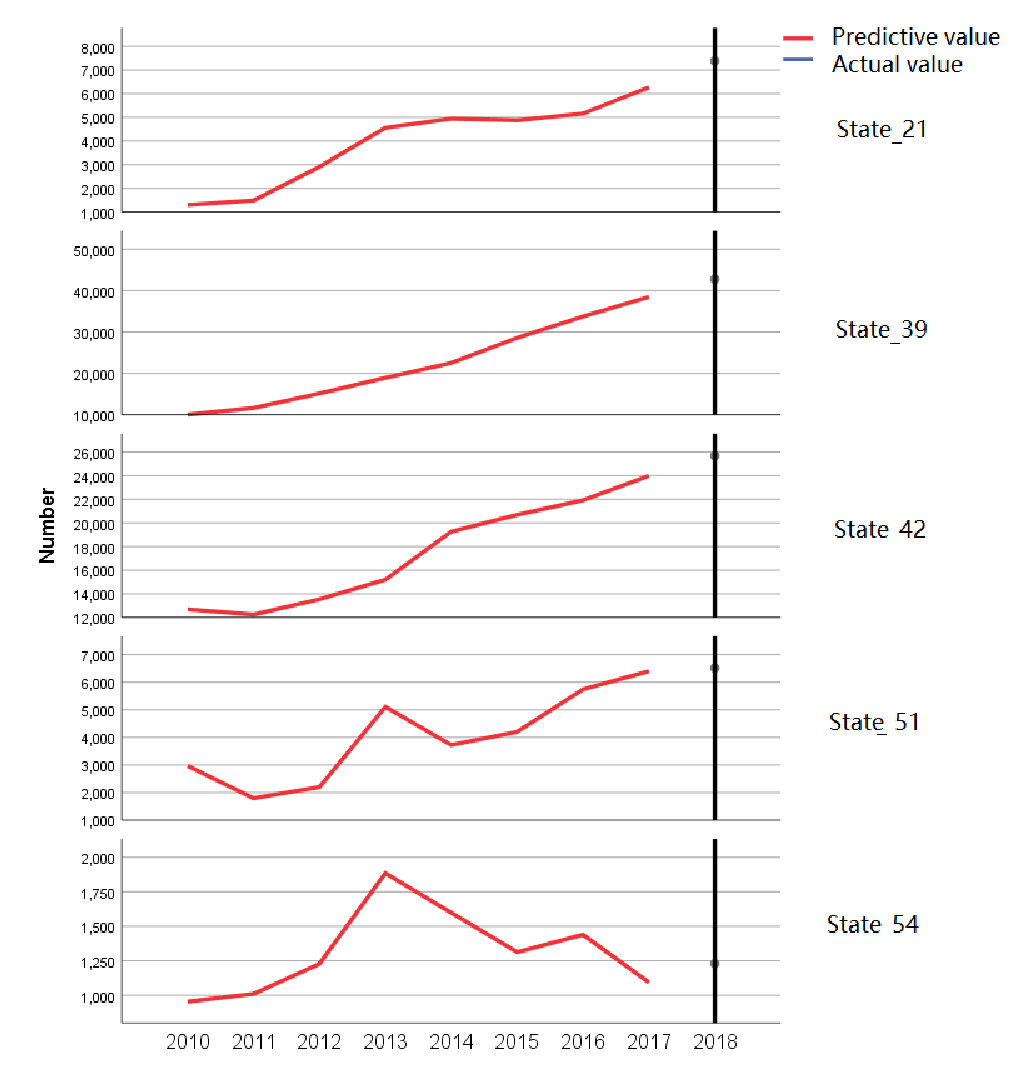
\includegraphics[width=0.8\textwidth]{figures/111.eps}
  \caption{Predicted Value in 2018}\label{2018}
\end{figure}\par
The data matrix is processed by interpolation and compared with the data of previous years to obtain the target matrix of BP neural network.\par
With the NNtool toolbox of MATLAB, a weight matrix W of $1\times 19$ is obtained.\par
As shown in Figure \ref{BPnn},the hidden layer has 10 neurons and the output layer has 1 output neuron. We subdivide the data given by Part 2 and get the training matrix of the neural network we built.\par
\begin{figure}[htbp]
  \centering
  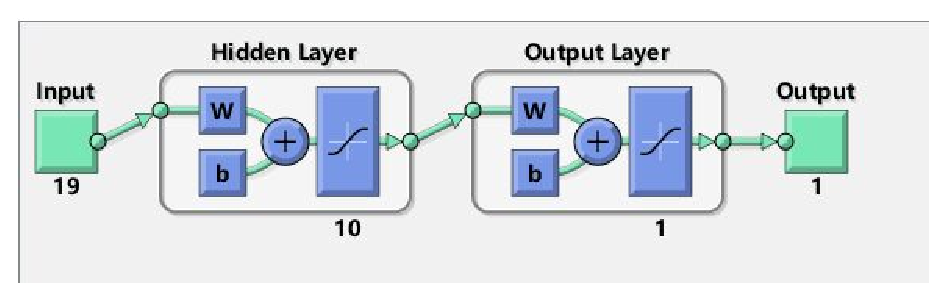
\includegraphics[width=\textwidth]{figures/nn.eps}
  \caption{BP Neural Network Diagram}\label{BPnn}
\end{figure}
For the neurons of the hidden layer, we get the weight matrix $W1 (10\times19)$: corresponding to it by the function of the matlab nntool toolbox:
$$W1=\left[
    \begin{array}{cccc}
      w1_{11}& w1_{12} & \cdots & w1_{1q_1} \\
      w1_{21} & w1_{22} & \cdots & w1_{2q_1}\\
      \vdots & \vdots &  & \vdots\\
      w1_{p_11} & w1_{p_12} & \cdots & w1_{p_1q_1} \\
    \end{array}
  \right]
(p_1=10,q_1=19) $$\par
Use a similar method to get the weight matrix of the output layer $W2 (1\times19)$:
$$W2=\left[
    \begin{array}{cccc}
      w1_{11}& w1_{12} & \cdots & w1_{1q_2} \\
    \end{array}
  \right]
(q_2=19) $$\par
For each indicator $x_i$, a weight matrix $W$ is obtained:
\begin{equation}\label{juzheng}
W=W2^T(X*W1)
\end{equation}
where,* means Hadamard product.
\subsection{Results of Model 2}

Using matlab for calculation, we get the weight matrix as shown in Table \ref{w1111}.
\begin{table}
  \centering
  \caption{Weight Matrix}\label{w1111}
  \begin{tabular}{|c|c|}
     \hline
indicator                                                                               & W       \\     \hline
Males Divorced                                                                          & 0.8796  \\
Total households                                                                        & 0.5295  \\
Less than 9th grade                                                                     & 0.5122  \\
\begin{tabular}[c]{@{}c@{}}Males \\   Separated\end{tabular}                            & 0.4098  \\
Males 15 years and over                                                                 & 0.3024  \\
Females Never married                                                                   & 0.199   \\
Some college, no degree                                                                 & 0.118   \\
Females 15 years and over                                                               & 0.098   \\
Graduate or professional degree                                                         & 0.0032  \\
Females Widowed                                                                         & -0.1114 \\
Females Divorced                                                                        & -0.2253 \\
\begin{tabular}[c]{@{}c@{}}High school graduate (includes\\   equivalency)\end{tabular} & -0.2475 \\
Females Separated                                                                       & -0.2545 \\
Associate's degree                                                                      & -0.3631 \\
Males Never married                                                                     & -0.378  \\
Males Widowed                                                                           & -0.3813 \\
Bachelor's degree                                                                       & -0.4421 \\
Nonfamily households                                                                    & -0.5906 \\
9th to 12th grade, no diploma                                                           & -0.7002\\     \hline
   \end{tabular}
\end{table}\par
It can be seen from the table that divorced men, low-educated people, and separated men have a high weight, that is, it is likely that they are abusing opioids.\par
In addition, the weight of total  households is also very high, indicating that family factors also have a great impact on opioids.
\section{Solution to the Opioids Crisis}
\subsection{Some Solutions to the Opioids Crisis}
Combining the results of the Part 1 and the Part 2, we give several solutions as follows:
\begin{enumerate}
  \item Promulgation of laws restricting the production of opioids (fundamental measures)
  \item Restrict the circulation of opioids between different regions (direct measures)
  \item Appropriately reduce the growth rate of the population
  \item Provide better education services
  \item Establish a community rehabilitation center
\end{enumerate}
\subsection{Program Feasibility Demonstration}
After the implementation of the above scheme, the model is used for prediction. The results obtained are shown in Table \ref{io}. (In actual operation, the policy is implemented by adjusting the value of the corresponding indicator."Before" in the table, data for 21 states in 2011.)\par
\begin{table}
  \centering
  \caption{Before and after policy implementation}\label{io}
  \begin{tabular}{|c|c|c|}
  \hline
Indicator             & Before  & After   \\\hline
1                     & 1681085 & 1581085 \\
2                     & 549670  & 559670  \\
3                     & 1687162 & 1587162 \\
4                     & 509862  & 519862  \\
5                     & 32002   & 22002   \\
6                     & 46532   & 56532   \\
7                     & 197189  & 187189  \\
8                     & 1783365 & 1683365 \\
9                     & 422346  & 412346  \\
10                    & 43653   & 53653   \\
11                    & 192110  & 202110  \\
12                    & 237722  & 247722  \\
13                    & 227766  & 217766  \\
14                    & 300804  & 310804  \\
15                    & 987495  & 1087495 \\
16                    & 577977  & 567977  \\
17                    & 192610  & 202610  \\
18                    & 353907  & 363907  \\
19                    & 240824  & 230824  \\\hline
Reports of drug abuse & 28285   & 20792\\\hline
\end{tabular}
\end{table}
It can be seen from the table that when the corresponding indicators change according to the expectations of the policy, the predicted number of abused Opioids is significantly reduced. It is proved that the policy is effective.
\section{Validating the Model}
In order to verify the correctness of the model, we use the 2010-2016 data to predict 2017 and compare it with the actual situation, and get the Table \ref{yanzheng}.\par
\begin{table}
  \centering  \caption{Model Verification}\label{yanzheng}
  \begin{tabular}{|c|c|c|c|c|c|}
\hline
State                 & 21    & 39    & 42    & 51    & 54    \\ \hline
2017 Predictive value & 6702  & 34698 & 25668 & 7112  & 1135  \\ \hline
2017 Actual value     & 6269  & 38482 & 23979 & 6398  & 1093  \\ \hline
Relative Error        & 0.069 & 0.098 & 0.070 & 0.112 & 0.038 \\ \hline
  \end{tabular}
\end{table}
As can be seen from the table, the prediction results are close to the actual values. For this set of data, the average relative error is 7.757\%
\section{Conclusions}
Through the above discussion, we have the following conclusions:
\begin{enumerate}
  \item The synthetic opioid and heroin have similar propagation characteristics.They are transmitted from a high concentration area to a low concentration area, while the concentration of high concentration area tends to be higher.
  \item When the number of opioids abuse reaches a threshold, the number of opioids will suddenly increase rapidly.
  \item Divorced men, low-educated people, and separated men are likely to abuse opioids. The abuse of opioids is also likely to occur in areas with large households.
  \item Taking corrective measures in a timely manner can reduce the harm caused by the abuse of opioids.
\end{enumerate}
\section{Evaluate of the Mode}
\subsection{Strengths}
\begin{itemize}
\item This model\textbf{ has a good point of innovation}, combining economic knowledge to link the dissemination of opioids with the production and sale of products.
\item After verification, \textbf{the accuracy of the model is high.}
\item The established models are connected and independent of each other, and \textbf{can work separately to improve efficiency.}
\end{itemize}
\subsection{Weaknesses}
\begin{itemize}
\item The model does not take into account the local drug retention and \textbf{may make the predictions slightly larger.}
\item The model does not take into account the geographical situation of each region.
\item In fact, there is a volatility in the ratio and the total quantity, and the model does not consider the difference between the two trends.
\end{itemize}
\section{Memo}
To the Chief Administrator:\par
Our team analyze the abuse of Opioids in an attempt to understand the seriousness of abuse of Opioids and how to address the abuse of Opioids.\par
By analyzing the 2010-2017 opioids abuse data and the 2010-2016 Census socio-economic data, we have obtained the following conclusions:
\begin{enumerate}
  \item \textbf{The propagation of opioids has certain characteristics.}\par Both the synthetic opioid and heroin have similar propagation characteristics, which are transmitted from a high concentration area to a low concentration area, while the concentration of high concentration area tends to be higher.\par At the same time, after our prediction, we believe that in 2018,Ohio is the most likely state of drug abuse in the future, both in synthetic opioids and in heroin.And,HAMILTON is the most prone to abuse of synthetic opioids, CUYAHOGA is second, MONTGOMERY is third;While MONTGOMERY is the most prone to heroin abuse, followed by LAKE, and the third is LUCAS.
\item \textbf{Indulging in opioids abuse is very dangerous.}\par When we continue to use our model to predict, we found that after 2022, when the total number of drug abuses in Ohio reached 275,040, both synthetic opioids and heroin suddenly exploded.
  \item \textbf{People who are abused by opioids can be foreseeable}\par Divorced men, low-educated people, and separated men are likely to abuse opioids. The abuse of opioids is also likely to occur in areas with large households.
  \item \textbf{The crisis caused by the abuse of opioids can be circumvented}\par Taking corrective measures in a timely manner can reduce the harm caused by the abuse of opioids.
\end{enumerate}
So, we made the following suggestions and hope that you can adopt them.\par
\begin{enumerate}
  \item  \textbf{Promulgation of laws restricting the production of opioids.}\par This is the fundamental way to solve the abuse of opioids, and it is the most effective method.
  \item \textbf{Restrict the circulation of opioids between different regions.}
  \item \textbf{Provide better education services}\par Reduce low-education, and educate people not to abuse opioids.
  \item \textbf{Establish a community rehabilitation center}\par Encourage people to treat diseases without the abuse of opioids
\end{enumerate}

Although the crisis brought by the abuse of opioids is severe, we believe that through joint efforts and reasonable measures, we can tide over the difficulties.\par Thank you!
\newpage
\begin{thebibliography}{99}\addcontentsline{toc}{section}{References}
\bibitem{wiki}\url{https://en.wikipedia.org/wiki/Opioid#Semisynthetic_and_synthetic_opioids}
\bibitem{computer virus} Feng Liping,Wang Hongbin,Feng Suqin.Improved SIR model of computer virus propagation in the network[J].Computer Applications,2011,31(07):1891-1893.
\bibitem{weight} Qiao Jiajun.Application of Improved Entropy Method in Sustainable Development Capacity Evaluation of Henan Province[J].Resources Science,2004(01):113-119.
\bibitem{ARIMA} Huang Wenling, Zheng Xiaoying, Breda McCarthy, Zhang Dabin. Short-term prediction of hog prices in Guangdong based on ARIMA model[J].Chinese Journal of Animal Science,2018,54(12):119-123.
\bibitem{zhuchengfen}\url{https://blog.csdn.net/u010480899/article/details/52263227?tdsourcetag=s_pctim_aiomsg}
\bibitem{BP} Liu Yujie,Chen Guiming,Liu Xiaofang,Zhan Jun.Study on BP Neural Network Weight and Threshold Initialization Method[J].Journal of Southwest China Normal University(Natural Science),2010,35(06):137-141.
\end{thebibliography}
\newpage
\begin{appendices}
\section{The Tables}
\begin{longtable}{|c|c|c|}
    \caption{Classification of Opioid}
    \label{table:opioid}  \\
    \hline
    &&\\

    \endfirsthead

    % Appear the table header at the top of every page
    \hline
    synthetic  opioid&non-synthetic opioid&others\\
  \hline
    \endhead

    % Appear \hline at the bottom of every page
    \hline
    \endfoot
synthetic  opioid             & non-synthetic opioid & others \\\hline
3,4-Methylenedioxy U-47700    & Acetyldihydrocodeine & Heroin \\
3-Fluorofentanyl              & Burenorphine         &        \\
3-Methylfentanyl              & Codeine              &        \\
4-Fluoroisobutyryl fentanyl   & Dihydrocodeine       &        \\
4-Methylfentanyl              & Hydrocodone          &        \\
Acetyl fentanyl               & Hydromorphone        &        \\
Acetylcodeine                 & Morphine             &        \\
Acryl fentanyl                & Oxycodone            &        \\
Alphaprodine                  & Oxymorphone          &        \\
ANPP                          & Thebaine             &        \\
Benzylfentanyl                &                      &        \\
Butorphanol                   &                      &        \\
Butyryl fentanyl              &                      &        \\
Carfentanil                   &                      &        \\
cis-3-methylfentanyl          &                      &        \\
Crotonyl fentanyl             &                      &        \\
Cyclopentyl fentanyl          &                      &        \\
Cyclopropyl fentanyl          &                      &        \\
Cyclopropyl/Crotonyl Fentanyl &                      &        \\
Desmethylprodine              &                      &        \\
Dextropropoxyphene            &                      &        \\
Dihydromorphone               &                      &        \\
Fentanyl                      &                      &        \\
Fluorobutyryl fentanyl        &                      &        \\
Fluorofentanyl                &                      &        \\
Fluoroisobutyryl fentanyl     &                      &        \\
Furanyl fentanyl              &                      &        \\
Furanyl/3-Furanyl fentanyl    &                      &        \\
Hydrocodeinone                &                      &        \\
Isobutyryl fentanyl           &                      &        \\
Levorphanol                   &                      &        \\
Meperidine                    &                      &        \\
Metazocine                    &                      &        \\
Methadone                     &                      &        \\
Methorphan                    &                      &        \\
Methoxyacetyl fentanyl        &                      &        \\
Mitragynine                   &                      &        \\
Morphine                      &                      &        \\
MT-45                         &                      &        \\
Nalbuphine                    &                      &        \\
o-Fluorofentanyl              &                      &        \\
Opiates                       &                      &        \\
Opium                         &                      &        \\
Pentazocine                   &                      &        \\
Pethidine                     &                      &        \\
p-Fluorobutyryl fentanyl      &                      &        \\
p-Fluorofentanyl              &                      &        \\
Phenyl fentanyl               &                      &        \\
p-methoxybutyryl fentanyl     &                      &        \\
Propoxyphene                  &                      &        \\
Remifentanil                  &                      &        \\
Tetrahydrofuran fentanyl      &                      &        \\
Tramadol                      &                      &        \\
trans-3-Methylfentanyl        &                      &        \\
U-47700                       &                      &        \\
U-48800                       &                      &        \\
U-49900                       &                      &        \\
U-51754                       &                      &        \\
Valeryl fentanyl              &                      &        \\
\hline
\end{longtable}
\newpage
\section{The Programmes}
Here are simulation programmes we used in our model as follow.\\

\textbf{\textcolor[rgb]{0.98,0.00,0.00}{Input matlab source:}}
\lstinputlisting[language=Matlab]{./code/shang.m}


\textcolor[rgb]{0.98,0.00,0.00}{\textbf{Input VBScript source:}}
\lstinputlisting[language=VBScript]{./code/divide_Excel.vbs}

\end{appendices}
\end{document}

%%
%% This work consists of these files mcmthesis.dtx,
%%                                   figures/ and
%%                                   code/,
%% and the derived files             mcmthesis.cls,
%%                                   mcmthesis-demo.tex,
%%                                   README,
%%                                   LICENSE,
%%                                   mcmthesis.pdf and
%%                                   mcmthesis-demo.pdf.
%%
%% End of file `mcmthesis-demo.tex'.
